%%%%%%%%%%%%%%%%%%%%%%%%%%%%%%%%%%%%%%%%%%%%%%%%%%%%%%%%%%%%%%%%%%%%%%%%%%%
\chapter{Technical Framework} 
%%%%%%%%%%%%%%%%%%%%%%%%%%%%%%%%%%%%%%%%%%%%%%%%%%%%%%%%%%%%%%%%%%%%%%%%%%%

One of the critical components in understanding and developing any system is establishing a firm theoretical framework. This chapter will delve into the foundational concepts and technologies that form the infrastructure of the HRMO system. By outlining the project code infrastructure, front-end and back-end technologies, and the database environment, the researchers aim to provide a comprehensive overview of the system's architecture and the rationale behind the technological choices. 

\section{Project Code Infrastructure}

    The web application utilizes Laravel by Taylor Otwell as the main full-stack web application framework. Laravel, by default, follows a Model-View-Controller (MVC) architectural pattern \cite{medium12023}. A common project structure when creating complex and dynamic web systems. 
    
    \begin{figure}[H]
        \centering
        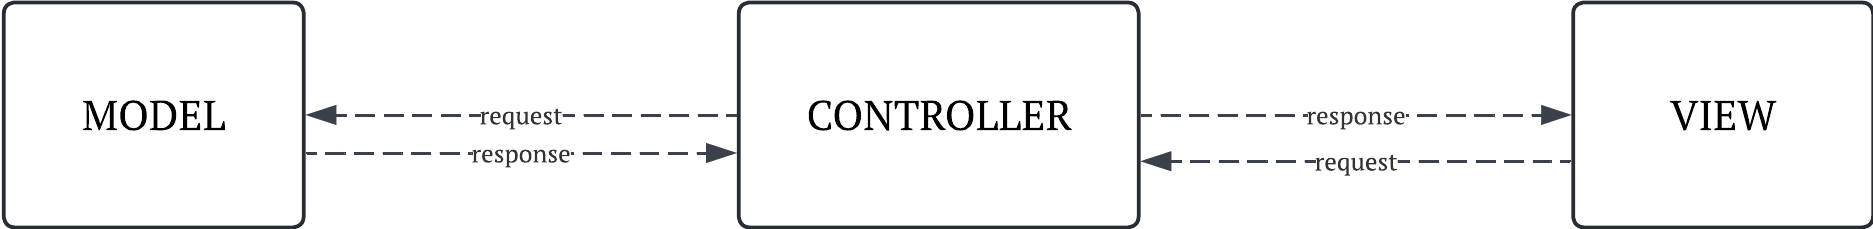
\includegraphics[width=1\linewidth]{figures/images/mvc.png}
        \caption{How the MVC Architecture Works.}
        \label{fig:enter-label}
    \end{figure}
    
    With this architecture, the process is streamlined and optimized by following the Single-Responsibility Principle (SRP) rule in programming. Wherein, the \textit{View} contains the web front-end web design/experience and logic for sending client requests to the server. For every request the client makes, is handled within the \textit{Controller}. Within this layer, it handles the logic for communicating within client-to-server requests and responses. Within this layer, will handle exceptions, validations, Data Access Objects (DAO), APIs, and many more \cite{mdn12023}.
    
    For every \textit{Controller} request to the Database, the \textit{Model} layer is responsible for interacting with the database. The \textit{Model} encapsulates the data and logic necessary for business operations, ensuring a clean separation of concerns. This architecture allows each component to focus on its specific responsibility, leading to a more maintainable and scalable system \cite{mdn12023} \cite{wikipedia12024}. 

\section{Development Tools and Technologies}

    To effectively build and maintain the project, different development tools and technologies are to be utilized. Among the key tools and technologies employed in the project's development lifecycle are the following:

    \begin{itemize}
        \item[] \textbf{Figma:} The developers utilized Figma as their main design tool to create high-fidelity wireframes, prototypes, and UI/UX designs. Figma offers a collaborative platform that enables seamless teamwork, version control, and real-time feedback among designers and stakeholders. 
        \item[] \textbf{Version Control Tools (Gitlab/Git):} The developers utilized version control tools such as Gitlab and Git to maintain version history and facilitate collaboration among team members. Git provides a distributed version control system that enables developers to track changes, manage code branches, and coordinate work effectively. Gitlab, as a web-based Git repository manager, offers additional features such as issue tracking, continuous integration (CI), and code review, enhancing the overall development workflow.
        \item[] \textbf{SQL Developer:} On the back-end side, SQL Developer is utilized within the application for developers to manage the database schema, execute queries, write procedures, and business logic to the application. This data accessibility is possible through the use of a Virtual Private Network (VPN) application approved by the University's Database Administrator (DBA) and Management Information Systems (MIS). With this, developers can establish a secure connection to the network, ensuring the confidentiality and integrity of data transmission between the application and the University's internal database.
    \end{itemize}

\subsection{Front-end Technologies and Languages}
    The system shall utilize different front-end technologies and languages to create a dynamic and responsive user interface. This will allow for a more streamlined development building complex features and modules. These technologies and languages will include:
    
    \begin{itemize}
        \item[] \textbf{NodeJS:} The application utilized NodeJS as its main runtime for running the front-end libraries. This decision allowed the developers to utilize and integrate the vast JavaScript ecosystem in the application e.g., Jquery, Bootstrap, Xtreme, etc.
        \item[] \textbf{Vite:} The application utilized Vite in partnership with NodeJS. This allowed the developers to efficiently increase productivity in development as Vite allows for fast Hot Module Reload (HRM). In addition, Vite is lightweight, fast, and efficient in alignment with the system's needs as it will be a high-traffic website.
        \item[] \textbf{Laravel Blade:} The application will utilize Laravel's built-in templating engine. Laravel's Blade supports writing dynamic HyperText Markup Language (HTML) with added Hypertext Preprocessor (PHP) accessibility and the capability to use static web languages such as HTML, Cascading Style Sheets (CSS), and JavaScript.
        \item[] \textbf{Laravel Livewire:} The application will utilize a front-end framework called Livewire. Livewire uses PHP as its main language and allows great compatibility with Laravel's default supported language. Livewire allows for building dynamic interfaces easily, without leaving the comfort of Laravel. By utilizing Livewire, the developers can write interactive components using simple PHP instead of relying heavily on JavaScript frameworks.
        \item[] \textbf{TailwindCSS:} The application utilized TailwindCSS as its main CSS Framework. TailwindCSS allows for efficient and ready-made utility classes in order to eliminate the use of writing CSS in the application. TailwindCSS allows for efficient space in the application as it purges unused styling upon production.
    \end{itemize}

\subsection{Back-end Technologies and Languages}
    The system will utilize back-end technologies in compatibility with Laravel's back-end framework support. These technologies and languages will include:
    
    \begin{itemize}
        \item[] \textbf{Laravel Livewire:} The application will utilize Livewire not only as a front-end framework but also as a tool to aid the controller in providing dynamic state changes in data requests. This allows for cleaner and shorter code for developers to write.
        \item[] \textbf{PHP:} The application shall utilize PHP as the main server scripting language for writing business logic throughout the entire system. PHP allows for robust server-side scripting, supported integration with Oracle Databases, and a wide range of frameworks and libraries that enhance development speed and efficiency. 
        \item[] \textbf{Composer:} The application will utilize Composer as its dependency manager for PHP. Composer allows for managing and installing libraries and packages efficiently, ensuring that all dependencies are up-to-date and compatible. With this, the developers can integrate third-party packages and tools to streamline the project setup.
      
    \end{itemize}

\subsection{Database Environment and Language}
    \begin{itemize}    
        \item[] \textbf{Oracle Database:} The application will utilize Oracle Database as its main Database Management System (DBMS). Oracle Database provides a robust, scalable, and secure environment for managing data \cite{oracle2nd}. By leveraging the Oracle Database, the application can handle large volumes of data efficiently and ensure high availability and reliability suitable for the project's complexity and objective capabilities.
        \item[] \textbf{PL/SQL:} The use of Oracle as a DBMS comes with built-in supported database languages such as the Structured Query Language (SQL) and Procedural Language extension to SQL (PL/SQL). With PL/SQL, developers can write powerful stored procedures and packages directly within the database. This enables efficient data processing and manipulation, as well as the implementation of business logic directly at the database level allowing for a more secure business logic processing and scalability \cite{oracle1nd}. 
    \end{itemize}